\documentclass[12pt]{article}
\usepackage[left=1cm, right=1cm, top=2cm,bottom=1.5cm]{geometry} 

\usepackage[parfill]{parskip}
\usepackage[utf8]{inputenc}
\usepackage[T2A]{fontenc}
\usepackage[russian]{babel}
\usepackage{enumitem}
\usepackage[normalem]{ulem}
\usepackage{amsfonts, amsmath, amsthm, amssymb, mathtools}
\usepackage{tabularx}
\usepackage{hhline}

\usepackage{accents}
\usepackage{fancyhdr}
\pagestyle{fancy}
\renewcommand{\headrulewidth}{1.5pt}
\renewcommand{\footrulewidth}{1pt}

\usepackage{graphicx}
\usepackage[figurename=Рис.]{caption}
\usepackage{subcaption}
\usepackage{float}

%%Наименование папки откуда забирать изображения
\graphicspath{ {./images/} }

%%Изменение формата для ввода доказательства
\renewcommand{\proofname}{$\square$  \nopunct}
\renewcommand\qedsymbol{$\blacksquare$}

%%Изменение отступа на таблицах
\addto\captionsrussian{%
	\renewcommand{\proofname}{$\square$ \nopunct}%
}
%% Римские цифры
\newcommand{\RN}[1]{%
	\textup{\uppercase\expandafter{\romannumeral#1}}%
}

%% Для удобства записи
\newcommand{\MR}{\mathbb{R}}
\newcommand{\MQ}{\mathbb{Q}}
\newcommand{\MN}{\mathbb{N}}
\newcommand{\MI}{\mathrm{I}}
\newcommand{\MJ}{\mathrm{J}}
\newcommand{\MH}{\mathrm{H}}
\newcommand{\MT}{\mathrm{T}}
\newcommand{\MU}{\mathcal{U}}
\newcommand{\MV}{\mathcal{V}}
\newcommand{\VN}{\varnothing}
\newcommand{\VE}{\varepsilon}

\theoremstyle{definition}
\newtheorem{defn}{Опр:}
\newtheorem{rem}{Rm:}
\newtheorem{prop}{Утв.}
\newtheorem{exrc}{Упр.}
\newtheorem{lemma}{Лемма}
\newtheorem{theorem}{Теорема}
\newtheorem{corollary}{Следствие}

\newenvironment{cusdefn}[1]
{\renewcommand\thedefn{#1}\defn}
{\enddefn}

\DeclareRobustCommand{\divby}{%
	\mathrel{\text{\vbox{\baselineskip.65ex\lineskiplimit0pt\hbox{.}\hbox{.}\hbox{.}}}}%
}
%Короткий минус
\DeclareMathSymbol{\SMN}{\mathbin}{AMSa}{"39}
%Длинная шапка
\newcommand{\overbar}[1]{\mkern 1.5mu\overline{\mkern-1.5mu#1\mkern-1.5mu}\mkern 1.5mu}
%Функция знака
\DeclareMathOperator{\sgn}{sgn}

%Обозначение константы
\DeclareMathOperator{\const}{\text{const}}

%Интеграл в большом формате
\DeclareMathOperator{\dint}{\displaystyle\int}

\newcommand{\smallerrel}[1]{\mathrel{\mathpalette\smallerrelaux{#1}}}
\newcommand{\smallerrelaux}[2]{\raisebox{.1ex}{\scalebox{.75}{$#1#2$}}}

\newcommand{\smallin}{\smallerrel{\in}}
\newcommand{\smallnotin}{\smallerrel{\notin}}

\newcommand*{\medcap}{\mathbin{\scalebox{1.25}{\ensuremath{\cap}}}}%
\newcommand*{\medcup}{\mathbin{\scalebox{1.25}{\ensuremath{\cup}}}}%

%Скалярное произведение
\DeclarePairedDelimiterX{\inner}[2]{\langle}{\rangle}{#1, #2}

%Подпись символов снизу
\newcommand{\ubar}[1]{\underaccent{\bar}{#1}}

\begin{document}
\lhead{Математический анализ - \RN{2}}
\chead{Шапошников С.В.}
\rhead{Лекция - 7}
\section*{Пространство ограниченных функций}

\begin{theorem}
	Если $f_n \in C^1[a,b]$, $f_n \overset{[a,b]}{\rightrightarrows} f$ и $f_n^\prime
	\overset{[a,b]}{\rightrightarrows} g$, тогда $g = f^\prime$.
\end{theorem}
\begin{rem}
	Несколько замечаний к доказательству:
	\begin{enumerate}[label ={(\arabic*)}]
		\item Из теоремы $\Rightarrow f \in C^1[a,b]$: равномерная сходимость сохраняет непрерывность $\Rightarrow f$ - непрерывна, $f^\prime = g \Rightarrow f$ - дифференцируема и поскольку производная является равномерным пределом непрерывных функций, то она сама является непрерывной функцией;
		\item Условие $f_n \overset{[a,b]}{\rightrightarrows} f$ можно заменить на условие: $\exists \, x_0 \in [a,b]\colon f_n(x_0)$ - сходится. Тогда утверждение будет звучать так: $\exists \, f \colon f_n \overset{[a,b]}{\rightrightarrows} f,\, f$ - дифференцируема и $f^\prime = g$. Почему возможна замена? Поскольку функции дифференцируема, то по теореме Лагранжа:
		$$
			\exists \, c \in [a,b]\colon (f_n(x) - f_m(x)) - (f_n(x_0) - f_m(x_0)) = (f_n^\prime(c) - f_m^\prime(c))(x - x_0) \Rightarrow 
		$$
		$$	
			\Rightarrow \forall x \in [a,b], \exists \, c \in [a,b]\colon f_n(x) - f_m(x) = (f_n^\prime(c) - f_m^\prime(c))(x - x_0) + (f_n(x_0) - f_m(x_0)) \Rightarrow
		$$	
		$$
			\Rightarrow \sup\limits_{[a,b]}|f_n(x) - f_m(x)| \leq |f_n(x_0) - f_m(x_0)| + \sup\limits_{[a,b]}|f_n^\prime(x) - f_m^\prime(x)|(b-a) \xrightarrow[]{n,m \to \infty}  0 
		$$
		\item В доказательстве не использовалась непрерывность $f_n^\prime$, поскольку это необходимо для простоты формулировки теоремы;
	\end{enumerate}
\end{rem}

\begin{corollary}
	Линейное пространство $C^k[a,b]$ ($k$-раз дифференцируемые функции, производные - непрерывны) с нормой 
	$$
		\|f \| = \max\limits_{[a,b]}|f| + \max\limits_{[a,b]}|f^\prime| + \dotsc + \max\limits_{[a,b]}|f^{(k)}|
	$$ 
	является банаховым пространством.
\end{corollary}
\begin{proof}
	Докажем для $k=1$, для более высоких порядков - аналогично. Факт, что $\|f\|$ - норма проверяется на семинарах.
	
	Пусть $f_n$ - фундаментальная последовательность, тогда:
	$$
		\forall \VE > 0, \exists \, N \colon \forall n,m > N,\, \|f_n -f_m\| < \VE \Rightarrow \max\limits_{[a,b]}|f_n - f_m| < \VE \wedge \max\limits_{[a,b]}|f_n^\prime - f_m^\prime| < \VE
	$$
	Тогда $f_n$ - фундаментальна в $C[a,b]$, а поскольку это полное пространство, то 
	$$
		\exists \, f \in C[a,b] \colon f_n \rightrightarrows f \Leftrightarrow \max\limits_{[a,b]}|f_n - f_m| \to 0
	$$ 
	
	Вместе с этим, $f_n^\prime$ - фундаментальна в $C[a,b]$. Тогда 
	$$ 
		\exists \, g \in C[a,b] \colon f_n^\prime \rightrightarrows g \Leftrightarrow
		\max\limits_{[a,b]}|f_n^\prime - g| \to 0
	$$
	Тогда по теореме: $f^\prime = g \Rightarrow f \in C^1[a,b]$. Тогда:
	$$
		\|f_n - f\| = \max\limits_{[a,b]}{|f_n - f|} + \max\limits_{[a,b]}{|f_n^\prime - f^\prime|} \to 0
	$$
	то есть, фундаментальная последовательность сходится.
\end{proof}
\newpage

Придумаем пример двух норм, которые не будут эквивалентными.

\textbf{Пример}: Пространство $C^1[a,b]$, $1$-ая норма: $\|f\|_0 = \max\limits_{[a,b]}|f|$, $2$-ая норма: $\|f\|_1 = \max\limits_{[a,b]}|f| + \max\limits_{[a,b]}|f^\prime|$. Эти нормы не являются эквивалентными. 

Нормы эквивалентны $\Leftrightarrow \exists \, c_1,c_2\colon \|\cdot\|_0 \leq c_1 \|\cdot\|_1 \wedge \|\cdot\|_1 \leq c_2 \|\cdot\|_0$. Но в данном случае, не выполняется второе неравенство.

Если $\|\cdot\|_1 \leq c_2 \|\cdot\|_0$, то $\max|f^\prime|$ оцениваете через $\max|f|$. Пусть $f_n(x) = \dfrac{1}{n}\sin{(n^2x)}$. Тогда $\max|f_n| \to 0$, но $f_n^\prime = n \cos{(n^2x)}$ и $\max|f_n^\prime| \to \infty$. То есть нормы не эквивалентны.

\section*{Открытые и замкнутые множества в метрических пространствах}
Пусть $(X, \rho)$ - метрическое пространство.

\begin{defn}
	Множество $\MU \subset X$ называется \uwave{открытым}, если $\forall a \in \MU, \, \exists \, B(a,r) \subset \MU$.
\end{defn}
\begin{defn}
	Множество $F \subset X$ называется \uwave{замкнутым}, если $X \setminus F$ - открытое.
\end{defn}

\textbf{Примеры}:\hfill
\begin{enumerate}[label ={(\arabic*)}]
	\item Открытый шар - открытое множество;
	\item Замкнутый шар - замкнутое множество;
\end{enumerate}
\begin{proof}\hfill
	\begin{enumerate}[label ={(\arabic*)}]
		\item Возьмем шар $B(a,r) = \{\,x \mid \rho(a,x) < r \,\}$, возьмем точку $b$ внутри этого шара, покажем, что она будет входить в $B(a,r)$ с некоторой своей окрестностью. 
		
		Пусть $\delta = r - \rho(a,b)$, возьмем шар $B(b,\delta)$. Проверим, что $\forall x \in B(b,\delta), \, x \in B(a,r)$:
		$$
			\rho(a,x) \leq \rho(a,b) + \rho(b,x) < \rho (a,b) + \delta = \rho(a,b) + (r - \rho(a,b)) = r
		$$
		\begin{figure}[H]
			\centering
			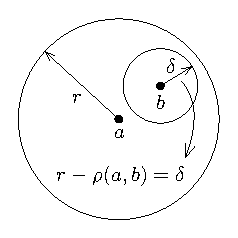
\includegraphics[width=0.25\textwidth]{7_1.eps}
			\caption{Открытый шар - открытое множество.}
			\label{7_1}
		\end{figure}
		\item (Упр.): Возьмем шар $\overline{B}(a,r) = \{\,x \mid \rho(a,x) \leq r \,\}$, покажем, что $X \setminus \overline{B}(a,r)$ - открытое множество. 
		
		Возьмем точку $b \notin \overline{B}(a,r)$, покажем, что она будет входить в $X \setminus\overline{B}(a,r)$ с некоторой своей окрестностью. 
		
		Поскольку $b \in X \setminus\overline{B}(a,r) \Rightarrow \rho(a,b) > r \Rightarrow$ пусть $\delta = \rho(a,b) - r > 0$, возьмем шар $B(b,\delta)$. Проверим, что $\forall x \in B(b,\delta), \, x \in X \setminus\overline{B}(a,r)$:
		$$
			\rho(a,b) \leq \rho(a,x) + \rho(x,b) \Rightarrow \rho(x,a) \geq \rho(a,b) - \rho(x,b) > \rho(a,b) - \delta = \rho(a,b) - \rho(a,b) + r = r
		$$
	\end{enumerate}
\end{proof}

\begin{prop}
	Пусть $(X,\|\cdot\|)$ и $F \subset X$ - конечномерное подпространство. Тогда $F$ - замкнуто.
\end{prop}
\begin{proof}
	Пусть $F = L(e_1, \dotsc, e_n)$, где $e_1, \dotsc, e_n$ - линейно независимые вектора, а $L$ - линейная оболочка, тогда 
	$$ 
		F = L(e_1,\dotsc, e_n) = \{\,c_1 e_1 + \dotsc + c_n e_n \,\}, \, c_i \in \MR
	$$
	
	Возьмем $a \notin F$, для доказательства достаточно найти шар $B(a,r) \colon B(a,r) \cap F = \VN$. 
	\begin{figure}[H]
		\centering
		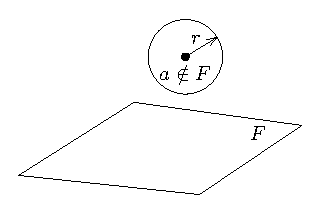
\includegraphics[width=0.25\textwidth]{7_2.eps}
		\caption{Шар $B(a,r) \colon B(a,r)\cap F = \VN$.}
		\label{7_2}
	\end{figure}
	Рассмотрим новое пространство: $F_{n+1} = L(e_1, \dotsc, e_n, e_{n+1}), \, e_{n+1} = a$, ясно, что они все линейно независимы, иначе $a$ выразился бы через $e_1, \dotsc, e_n$ и тогда бы $a \in F$, но $a \notin F$. Тогда:
	$$
		\forall x \in F_{n+1},\, x = c_1 e_1 + \dotsc + c_n e_n + c_{n+1} e_{n+1}, \, c_i \in \MR
	$$
	Введем на этом пространстве норму (проверка, что это норма - точно такая же, как и в $\MR^n$ для координат): 
	$$
		\|x\|_2 = \sqrt{c_1^2 + \dotsc + c_n^2 + c_{n+1}^2}
	$$
	По этой норме, каково расстояние от векторов $e_{n+1}$ до рассматриваемой плоскости $F$? 
	
	$F = \{\,c_{n+1} = 0 \,\}$ в пространстве $F_{n+1 }$ ($F \subset F_{n+1}$). Пусть $x = (c_1, \dotsc, c_n, 0) \in F$, тогда 
	$$
		e_{n+1} = (0,\dotsc, 0,1) \Rightarrow \|x - e_{n+1}\|_2 = \sqrt{c_1^2 + \dotsc + c_n^2 + 1^2} \geq 1 
	$$
	Если взять множество $\{\,x \in F_{n+1} \colon \|x - e_{n+1}\|_2 < 1 \,\}$, то оно не будет пересекаться с $F$. 
	
	Так как $F_{n+1}$ - конечномерно, то $\|\cdot\|_2$ эквивалентно исходной норме $\| \cdot \|$ на $F_{n+1}$, в частности 
	$$
		\exists \, C > 0 \colon \|\cdot \|_2 \leq C \|\cdot \|
	$$
	
	Шар $B\big(e_{n+1}, \tfrac{1}{C}\big) \cap F_{n+1} \subset \{\,x \in F_{n+1}\colon \|x - e_{n+1} \|_2 < 1  \,\}$ и, следовательно, не пересекается с $F \Rightarrow$
	$$
		B\big(e_{n+1}, \tfrac{1}{C}\big) \cap F = \VN
	$$
\end{proof}

\begin{exrc}
	Показать на примере, что конечномерность важна (привести пример линейного подпространства, которое бесконечномерно, но не является замкнутым). 
\end{exrc}
\subsection*{Свойства открытых и замкнутых множеств}
\begin{theorem} 
	Верны следующие свойства:
	\begin{enumerate}[label ={(\arabic*)}]
		\item Объединение всякого набора открытых множеств и пересечение конечного набора открытых множеств, является открытым множеством;
		\item Пересечение всякого набора замкнутых множеств и объединение конечного набора замкнутых множеств, является замкнутым множеством;
	\end{enumerate}
\end{theorem}
\begin{proof}
	\begin{enumerate}[label ={(\arabic*)}]
		\item Пусть $\{\MU_\alpha\}$ - набор открытых множеств, возьмем точку $a \in \textstyle \bigcup\limits_{\alpha}\MU_\alpha \Rightarrow \exists \, \alpha_0 \colon a \in \MU_{\alpha_0} \Rightarrow$ 
		$$
			\exists \, B(a,r)\subset \MU_{\alpha_0} \Rightarrow B(a,r) \subset \textstyle \bigcup\limits_{\alpha}\MU_\alpha
		$$
		Таким образом, объединение всякого набора открытых множеств является открытым множеством.
		
		Пусть $\{\MU_1,\dotsc, \MU_N\}$ - набор открытых множеств, возьмем точку $a \in \textstyle \bigcap\limits_{k = 1}^{N}\MU_k \Rightarrow a \in \MU_k, \, \forall k \Rightarrow$
		$$
			\forall k,\, \exists \, B(a,r_k)\subset \MU_k \Rightarrow r = \min\{r_1,\dotsc, r_N\} \Rightarrow \forall k,\, B(a,r) \subset \MU_k \Rightarrow B(a,r) \subset \textstyle \bigcap\limits_{k = 1}^{N}\MU_k
		$$
		Таким образом, пересечение конечного набора открытых множеств является открытым множеством;
		\item \uline{Указание}: $X \setminus F$ - открытое множество и используем формулу Моргана (см. прошлый семестр);
	\end{enumerate}
\end{proof}
\begin{rem}
	Всякое открытое множество есть объединение открытых шаров:
	$$
		\MU = \textstyle\bigcup\limits_{a \smallin \MU}B(a,r)
	$$
\end{rem}
\newpage
\section*{Топология точек множества метрического пространства}
Пусть $(X, \rho)$ - метрическое пространство и $A \subset X$.
\begin{defn}
	Точка $a \in A$ называется \uwave{внутренней}, если $\exists \, B(a,r)\subset A$.
\end{defn}
\begin{rem}
	В открытом множестве все точки - внутренние.
\end{rem}
\begin{defn}
	Точка $a$ называется \uwave{граничной}, если $\forall B(a,r),\, B(a,r) \cap A \neq \VN \wedge B(a,r) \cap (X \setminus A) \neq \VN$.
\end{defn}
\begin{defn}
	Точка $a$ называется \uwave{предельной} (для множества $A$), если $\forall B(a,r),\, B(a,r) \cap A$ - бесконечное множество.
\end{defn}
\begin{defn}
	\uwave{Проколотый шар} с центром в точке $a$ радиуса $r$ это множество: $B^\prime(a,r) = B(a,r) \setminus \{a\}$.
\end{defn}

\begin{prop}
	Точка $a$ - предельная точка множества $A \Leftrightarrow \forall B(a,r),\, B^\prime(a,r) \cap A \neq \VN$.
\end{prop}
\begin{proof}\hfill\\
	$(\Rightarrow)$ Очевидно, так как выкидывание одной точки из бесконечного множества ни на что не влияет и $\forall B(a,r),\, B^\prime(a,r) \cap A \neq \VN$.
	
	$(\Leftarrow)$ (От противного): Пусть точка $a \colon \forall B(a,r),\, B^\prime(a,r) \cap A \neq \VN$ - не является предельной точкой, тогда $\exists \, B^\prime(a,r_0)$ в котором лежит не более, чем конечное множество точек из $A$: $B(a,r_0) \cap A$ - конечное множество. 
	\begin{figure}[H]
		\centering
		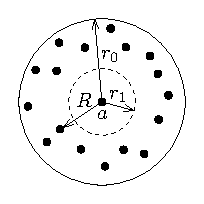
\includegraphics[width=0.15\textwidth]{7_3.eps}
		\caption{Уменьшение шара.}
		\label{7_3}
	\end{figure}
	Пусть $R = \min\limits_{x \in C}{\rho(a,x)}, \, C = B^\prime(a,r_0)\cap A \Rightarrow$ уменьшим радиус шара таким образом, что $r_1 < R \Rightarrow B^\prime(a,r_1) \cap A = \VN \Rightarrow$ противоречие.
\end{proof}

\begin{theorem}
	Следующие утверждения равносильны:
	\begin{enumerate}[label ={\arabic*)}]
		\item $A$ - замкнуто;
		\item $A$ содержит все свои граничные точки;
		\item $A$ содержит все свои предельные точки;
		\item Если $a_n \in A$ и $a_n \to a$, то $a \in A$;
	\end{enumerate}
\end{theorem}
\begin{proof}\hfill\\
	$1) \Rightarrow 2)$ Пусть $a$ - граничная точка $A$, предположим, что $a \notin A$, так как $A$ замкнуто, то $X \setminus A$ - открытое множество $\Rightarrow \exists \, B(a,r) \colon B(a,r)\cap A = \VN \Rightarrow$ противоречие с определением граничной точки.
	\begin{figure}[H]
		\centering
		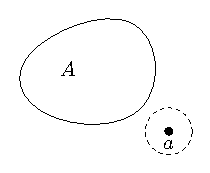
\includegraphics[width=0.25\textwidth]{7_4.eps}
		\caption{В шаре $B(a,r)$ нет точек из $A \Rightarrow$ противоречие с определением граничной точки.}
		\label{7_4}
	\end{figure}
	$2) \Rightarrow 3)$ Пусть $a$ - предельная точка $A$, предположим, что $a \notin A$, тогда $a$ - граничная, так как для предельной точки в её окрестности есть бесконечно много точек из $A$ и сама точка $a \notin A$. Но все граничные точки должны $\in A \Rightarrow$ противоречие.
	\begin{figure}[H]
		\centering
		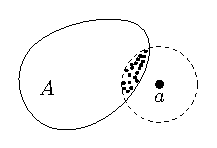
\includegraphics[width=0.25\textwidth]{7_5.eps}
		\caption{Точка $a \notin A$ - предельная $\Rightarrow$ это граничная точка $\Rightarrow a\in A \Rightarrow$ противоречие.}
		\label{7_5}
	\end{figure}
	$3) \Rightarrow 4)$ Возьмем последовательность точек $a_n \in A, \, a_n \to a$. Если $\exists \, n \colon a_n = a \Rightarrow$ выполнено. 
	
	Если $\forall n, \, a_n \neq a$, тогда $a$ - предельная точка, поскольку $a_n \to a \Rightarrow$ в любой проколотой окрестности $B^\prime(a,r)$ найдутся точки из $a_n \Rightarrow a \in A$.
	\begin{figure}[H]
		\centering
		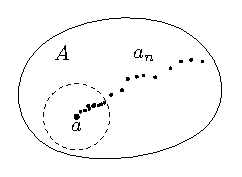
\includegraphics[width=0.25\textwidth]{7_6.eps}
		\caption{ $\forall n, \, a_n \neq a$, тогда $a$ - предельная точка $\Rightarrow a \in A$.}
		\label{7_6}
	\end{figure}
	$4) \Rightarrow 1)$ Предположим, что $X \setminus A$ не является открытым, тогда возьмем точку $a \in X \setminus A$, такую что не существует окрестности с центром в $a$, которая целиком бы лежала в $X \setminus A$:
	$$
		\forall B\big(a,\tfrac{1}{n}\big), \, \exists \, a_n \in B\big(a,\tfrac{1}{n}\big)
	$$	
	\begin{figure}[H]
		\centering
		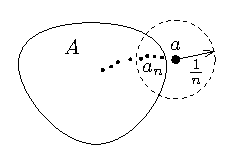
\includegraphics[width=0.25\textwidth]{7_7.eps}
		\caption{ Точки $a_n \in B\big(a,\tfrac{1}{n}\big) \Rightarrow a_n \to a \Rightarrow a \in A \Rightarrow$ противоречие.}
		\label{7_7}
	\end{figure}
	Тогда получим последовательность $a_n \in A \colon  \rho(a_n,a) \to 0 \Rightarrow a_n \to a \Rightarrow a \in A \Rightarrow$ противоречие.
\end{proof}

\begin{defn}
	Множество $\overline{A} = A \cup \{\text{граничные точки } A\}$, называется \uwave{замыканием} множества $A$.
\end{defn}

\begin{prop}
	Следующие утверждения верны:
	\begin{enumerate}[label ={\arabic*)}] 
		\item $\overline{A}$ - замкнутое множество;
		\item $\overline{A}$ - наименьшее замкнутое множество, содержащее $A$:  $\overline{A} =  \bigcap\limits_{A \subset F}F \vspace{-\parskip}$, где $F$ - замкнутые;
		\item $A$ - замкнуто $\Leftrightarrow A = \overline{A}$;
	\end{enumerate}
\end{prop}
\begin{proof}\hfill
	\begin{enumerate}[label ={\arabic*)}]
		\item Пусть $b$ - граничная точка $\overline{A} \Rightarrow$ в любой окрестности точки $b$ будет точка из $\overline{A}$. По определению, $\overline{A}$ содержит два типа точек: либо это точка из $A$, либо это граничная точка $A$. 
		
		В случае, когда это граничная точка из $A \Rightarrow$ можно взять окрестность этой точки, внутри окрестности точки $b$ и она обязательно будет содержать точки из $A$ (как граничная точка из $A$). 
		\begin{figure}[H]
			\centering
			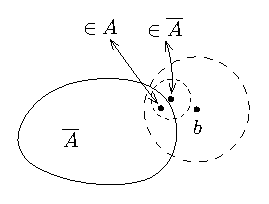
\includegraphics[width=0.3\textwidth]{7_8.eps}
			\caption{$b$ - граничная точка $\overline{A} \Rightarrow$ если $\exists$ граничная точка $A \Rightarrow$ в её окрестности найдем точку из $A$.}
			\label{7_8}
		\end{figure}
		Таким образом, в любой окрестности точки $b$ есть точки из $A$ и точки не из $\overline{A}$ (поскольку это граничная точка) $\Rightarrow b$ - граничная точка $A$ и $b \in \overline{A}$;
		
		\item Надо проверить, что в любом замкнутом множестве лежит $\overline{A} \Rightarrow$ если $F$ - замкнуто и $A\subset F \Rightarrow$ граничные точки $A \subset F$.
		
		Пусть $a \notin F$ - граничная точка $A \Rightarrow$ так как, в любой окрестности есть элементы из $A \subset F$, а сама точка не из $F$, то $a$ - граничная для $F$ и должна в $F$ лежать (так как, $F$ - замкнутое множество);
		\begin{figure}[H]
			\centering
			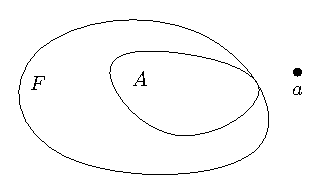
\includegraphics[width=0.3\textwidth]{7_9.eps}
			\caption{$a \notin F$ - граничная точка $A \Rightarrow$ в её окрестности есть элементы из $A \Rightarrow a$ - граничная для $F$.}
			\label{7_9}		
		\end{figure}
		\item Уже доказали - смотри выше теорему. Если $A$ замкнуто, то оно содержит все свои граничные точки $\Rightarrow A = \overline{A}$. И наоборот, если $A$ содержит все свои граничные точки, то $A$ - замкнуто;
	\end{enumerate}
\end{proof}

\end{document}